
\documentclass[]{hdsr}

%Graphics should all go in the figs/ directory
\graphicspath{{figs/}}

\begin{document}

\begin{center}

\title{Pythagorean theorem}
\author{M.Amin Roshani}
\date{\today}
\maketitle

\end{center}
\tableofcontents
\newpage


% Larger bottom margin for the first page
\newgeometry{bottom=1.5in}


\begin{center}

\end{center}


\section*{Abstract}
In mathematics, the Pythagorean theorem, also known as Pythagoras' theorem, is a fundamental relation in Euclidean geometry among the three sides of a right triangle. It states that the area of the square whose side is the hypotenuse (the side opposite the right angle) is equal to the sum of the areas of the squares on the other two sides. This theorem can be written as an equation relating the lengths of the sides a, b and c, often called the "Pythagorean equation".

\section{Rearrangement proof}
\label{sec1}
The two large squares shown in the figure each contain four identical triangles, and the only difference between the two large squares is that the triangles are arranged differently. Therefore, the white space within each of the two large squares must have equal area. Equating the area of the white space yields the Pythagorean theorem, Q.E.D.\cite{3}

Heath gives this proof in his commentary on Proposition I.47 in Euclid's Elements, and mentions the proposals of Bretschneider and Hankel that Pythagoras may have known this proof. Heath himself favors a different proposal for a Pythagorean proof, but acknowledges from the outset of his discussion "that the Greek literature which we possess belonging to the first five centuries after Pythagoras contains no statement specifying this or any other particular great geometric discovery to him." Recent scholarship has cast increasing doubt on any sort of role for Pythagoras as a creator of mathematics, although debate about this continues.
\begin{figure}[H]
    \centering
    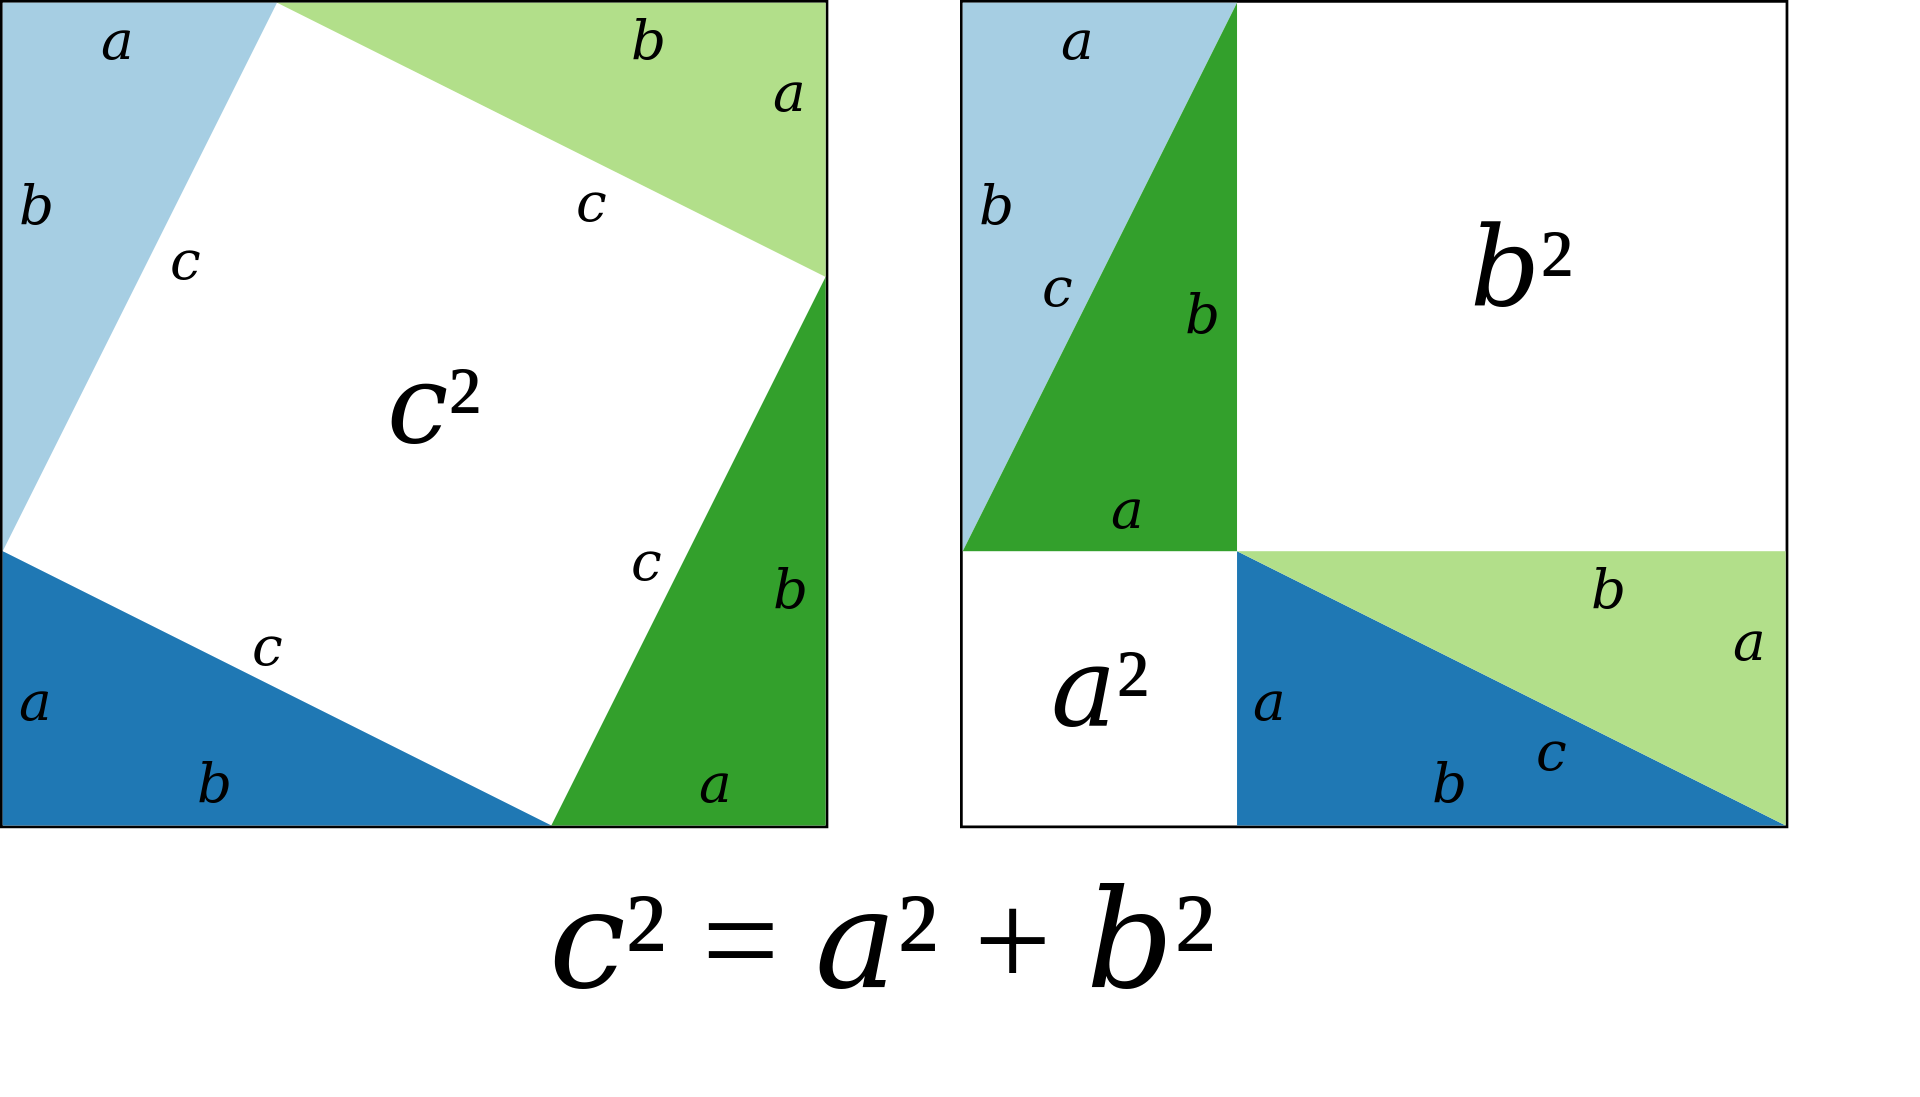
\includegraphics[scale=0.15]{Pythagoras-proof-anim.svg.png} \\
    \caption{The rearrangement proof}
    \label{fig:my_label}
\end{figure}
\begin{equation}
    c = \sqrt{a^2 + b^2}
\end{equation}
\begin{equation}
    \sqrt{(a_1 + a_1)^2 + (a_2 + a_2)^2 + (a_n + a_n)^2} = \sqrt{\sum_{i=1}^{n} (a_i - b_i)^2}
\end{equation}
\subsection{Extra explanation}

The Pythagorean equation relates the sides of a right triangle in a simple way, so that if the lengths of any two sides are known the length of the third side can be found. Another corollary of the theorem is that in any right triangle, the hypotenuse is greater than any one of the other sides, but less than their sum.


\section{Other proofs of the theorem}
Albert Einstein gave a proof by dissection in which the pieces need not get moved. Instead of using a square on the hypotenuse and two squares on the legs, one can use any other shape that includes the hypotenuse, and two similar shapes that each include one of two legs instead of the hypotenuse (see Similar figures on the three sides). In Einstein's proof, the shape that includes the hypotenuse is the right triangle itself. The dissection consists of dropping a perpendicular from the vertex of the right angle of the triangle to the hypotenuse, thus splitting the whole triangle into two parts. Those two parts have the same shape as the original right triangle, and have the legs of the original triangle as their hypotenuses, and the sum of their areas is that of the original triangle. Because the ratio of the area of a right triangle to the square of its hypotenuse is the same for similar triangles, the relationship between the areas of the three triangles holds for the squares of the sides of the large triangle as well.

% 1. When figure position is crucial, use the [H] tag 
%    to enforce absolute positioning
% 2. Image files should be referenced without file extension
\section{List of some proofs}
\begin{enumerate}
     \item Proof using similar triangles
    \item Euclid's proof
    \item Proofs by dissection and rearrangement
    \item Einstein's proof by dissection without rearrangement
    \item Algebraic proofs
\end{enumerate}


\subsection{Table of proofs}
\begin{center}
 \begin{tabular}{||c | c||} 
\hline
 1 & Proof using similar triangles \\ 
 \hline
 2 & Euclid's proof \\
 \hline
 3 & Proofs by dissection and rearrangement \\
 \hline
 4 & Einstein's proof by dissection without rearrangement \\
 \hline
 5 & Algebraic proofs \\ [1ex] 
 \hline
\end{tabular}
\newline
\end{center}

    \begin{thebibliography}{1}

        \bibitem{1}item {
            Judith D. Sally; Paul Sally (2007). "Chapter 3: Pythagorean triples". Roots to research: a vertical development of mathematical problems. American Mathematical Society Bookstore. p. 63. ISBN 0-8218-4403-2.}
        \bibitem{2}item {
             Benson, Donald. The Moment of Proof : Mathematical Epiphanies, pp. 172–173 (Oxford University Press, 1999).}
        \bibitem{3}item {
            Huffman, Carl. "Pythagoras". In Zalta, Edward N. (ed.). The Stanford Encyclopedia of Philosophy (Winter 2018 Edition)., "It should now be clear that decisions about sources are crucial in addressing the question of whether Pythagoras was a mathematician and scientist. The view of Pythagoras' cosmos sketched in the first five paragraphs of this section, according to which he was neither a mathematician nor a scientist, remains the consensus."}
    \end{thebibliography}


\end{document}
